\subsection{Running an Caesar Program}
Select your Caesar project in the Package Explorer. Drop-down the \markedtext{Run} icon on the toolbar and click \markedtext{Run...}\\
Select \markedtext{Java Application} in the left-hand tab and click \markedtext{New}.
Name this configuration \code{HelloWorld} and then click \markedtext{Search} to find the main class. Select \code{HelloWorld} as described in figure \ref{fig:run}.

\begin{figure*}[htbp]
	\centering
		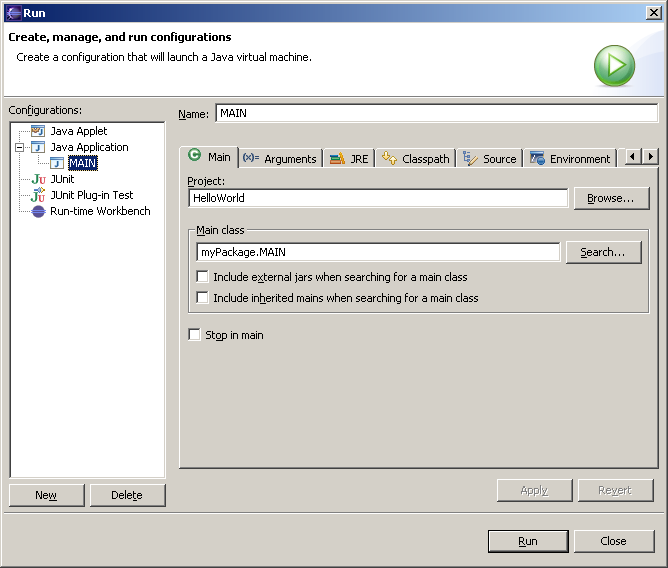
\includegraphics[width=0.80\textwidth]{images/run.png}
	\caption{Running a \caesarj ~program}
	\label{fig:run}
\end{figure*}

Click \markedtext{Apply} and then \markedtext{Run}.\\
You should see the output of the \code{HelloWorld} ~class and the \code{World} ~aspect in the console like shown in figure \ref{fig:console}.

\begin{figure*}[htbp]
	\centering
		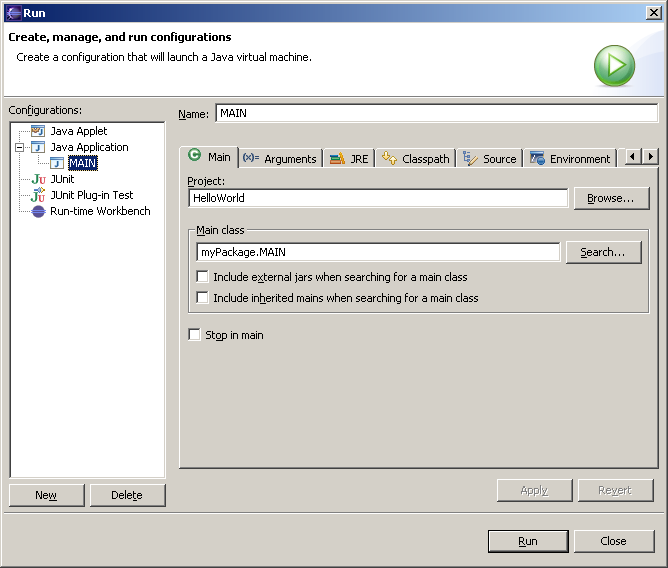
\includegraphics[width=0.80\textwidth]{images/run.png}
	\caption{Programs output}
	\label{fig:console}
\end{figure*}
To run this configuration again, just click on the \markedtext{Run} icon placed on the toolbar.
